\documentclass[12pt, a4paper]{article}
% !TEX program = xelatex
% Instructions:
% 1. VSCode + LaTeX Workshop plugin is recommended for editing and compiling this LaTeX document. You can also use any LaTeX editor of your choice.
% 2. Compilation engine: Please select XeLaTeX (to support Times New Roman font).
% 3. mbi6013.sty is a custom style file provided for this course. Make sure it is in the same directory as this main.tex file.

\usepackage{mbi6013}

\begin{document}

% ==========================================
% Title Page
% ==========================================
\begin{titlepage}
    \centering
    \vspace*{2cm}

    {\LARGE \bfseries Research Proposal: The Title\par}
    
    \vspace{3cm}
    
    {\Large \textbf{Student ID:} 2250500xx\par}
    \vspace{0.5cm}
    {\Large \textbf{Student Name:} guwudx\par}
    \vspace{0.5cm}
    {\Large \textbf{Mentor:} Prof. Yongfei Wang\par} 
    \vspace{0.5cm}
    {\Large \textbf{Course Instructor:} Prof. Yongfei Wang\par} 
    \vspace{0.5cm}
    {\Large \textbf{Department:} School of Medicine, MSC in Bioinformatics\par}
    \vspace{0.5cm}
    {\Large \textbf{Institution:} The Chinese University of Hong Kong, Shenzhen\par}
    
    \vfill
    
    {\large \today\par}
\end{titlepage}

\newpage

% ==========================================
% A. Background and Significance
% ==========================================
\section*{A. Background and Significance}
\addcontentsline{toc}{section}{A. Background and Significance}

This section will provide a comprehensive overview of the current state of research in the field, highlighting the gaps and challenges that our proposed study aims to address. We will discuss the significance of our research question and how it contributes to advancing knowledge in the area. Additionally, we will review relevant literature to establish the context for our specific aims and research design. We will also emphasize the potential impact of our findings on both the scientific community and [Add your specific biological significance here], unders ...

% ==========================================
% B. Specific Aims
% ==========================================
\section*{B. Specific Aims}
\addcontentsline{toc}{section}{B. Specific Aims}

The long-term objective of this research is to establish.... To test the central hypothesis that ... , we propose the following specific aims:

\begin{itemize}[leftmargin=*]
    \item \textbf{Aim 1: To ...} We will test/construct/verify a ...
    \item \textbf{Aim 2: To ...} We will implement a ...
    \item \textbf{Aim 3 (Optional): [Short Title of Aim 3]} Describe a third aim if necessary (2-3 aims recommended).
\end{itemize}

% ==========================================
% C. Preliminary Data
% ==========================================
\section*{C. Preliminary Data}
\addcontentsline{toc}{section}{C. Preliminary Data}

At this conceptual stage, extensive data collection is ongoing. However, preliminary analyses have yielded promising insights. For instance, we have observed that ... (insert any early findings or pilot data that support the feasibility of the proposed research). These initial results provide a strong foundation for the proposed specific aims and suggest that our approach is viable.

% ==========================================
% D. Research (Experimental) Design and Methods
% ==========================================
\section*{D. Research (Experimental) Design and Methods}
\addcontentsline{toc}{section}{D. Research Design and Methods}

\subsection*{D.1 Underlying Methodology and Rationale}
\subsubsection*{Overview}
This section outlines the methodological framework underlying our proposed research. We employ a multi-stage approach integrating computational and experimental methods to achieve our specific aims.

\subsubsection*{Rationale}
Our methodology is grounded in established principles from the field, adapted to address the unique challenges identified in Section A. This approach allows us to systematically test our central hypothesis while maintaining scientific rigor and reproducibility.

\subsubsection*{Key Methods}
We will utilize [specify primary methods/techniques]. This choice is justified because [provide rationale]. Our approach builds upon [reference preliminary data or existing literature], ensuring feasibility and relevance to our research objectives.

\textbf{Bold Font:} As illustrated in \ref{fig:wgt}, it ...

\begin{figure}[H]
    \centering
    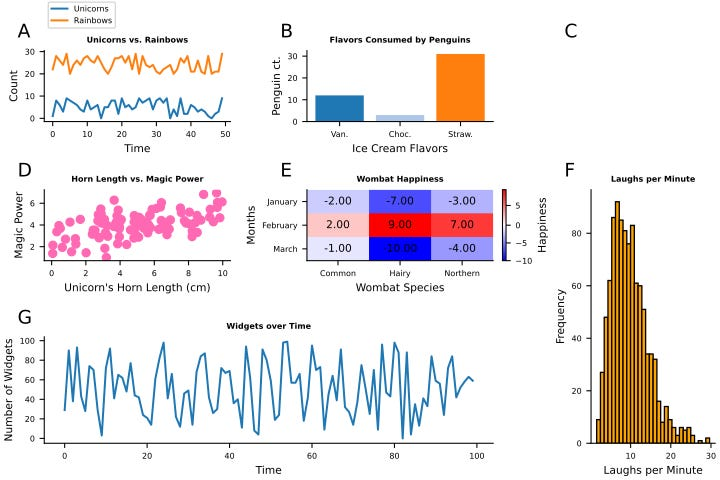
\includegraphics[width=0.85\textwidth]{assets/example.png}
    \caption{This is a simple figure. Replace this caption with a descriptive caption relevant to your research.}
    \label{fig:wgt}
\end{figure}

\subsection*{D.2 Data Analysis and Interpretation}
Data analysis will be conducted using [specify software/tools]. We will apply [describe statistical methods or computational techniques] to analyze the data collected from our experiments. The interpretation of results will be guided by our central hypothesis and the specific aims outlined in Section B. We will also perform sensitivity analyses to assess the robustness of our findings and explore potential confounding factors.

\subsection*{D.3 Potential Difficulties and Alternative Approaches}
While we have designed our research to minimize potential difficulties, we acknowledge that challenges may arise. For instance, if [describe a potential issue], we will implement [describe an alternative approach]. Additionally, we will conduct regular reviews of our methodology and data to identify any unforeseen issues early on and adjust our approach accordingly.

\subsection*{D.4 Timetable}
\begin{itemize}
    \item \textbf{Month 1-2:} Data collection and preliminary analysis.
    \item \textbf{Month 3-4:} Method development and validation.
    \item \textbf{Month 5-6:} Comprehensive data analysis and interpretation.
    \item \textbf{Month 7-8:} Manuscript preparation and submission
\end{itemize}

% ==========================================
% E. Bibliography or Reference List
% ==========================================
\newpage
\section*{E. Bibliography or Reference List}
\addcontentsline{toc}{section}{E. Bibliography}

[Bibliography will be inserted here via Zotero integration or edit by hand.]

\end{document}